\section*{Úvod}

FSK modulace je založená na technice frekvenčního klíčování. Funguje to tak, že jednotlivým vysílaným symbolům (0, 1) odpovídá harmonický signál o definované frekvenci.

Realizovaný systém si klade za cíl demodulovat a posléze dekódovat správy vysílané modemem BEL202. Úrovni logické jedničky odpovídá kmitočet $1,2~kHz$ a logické nule $2,2~kHz$.

\begin{figure}[H]
    \centering
    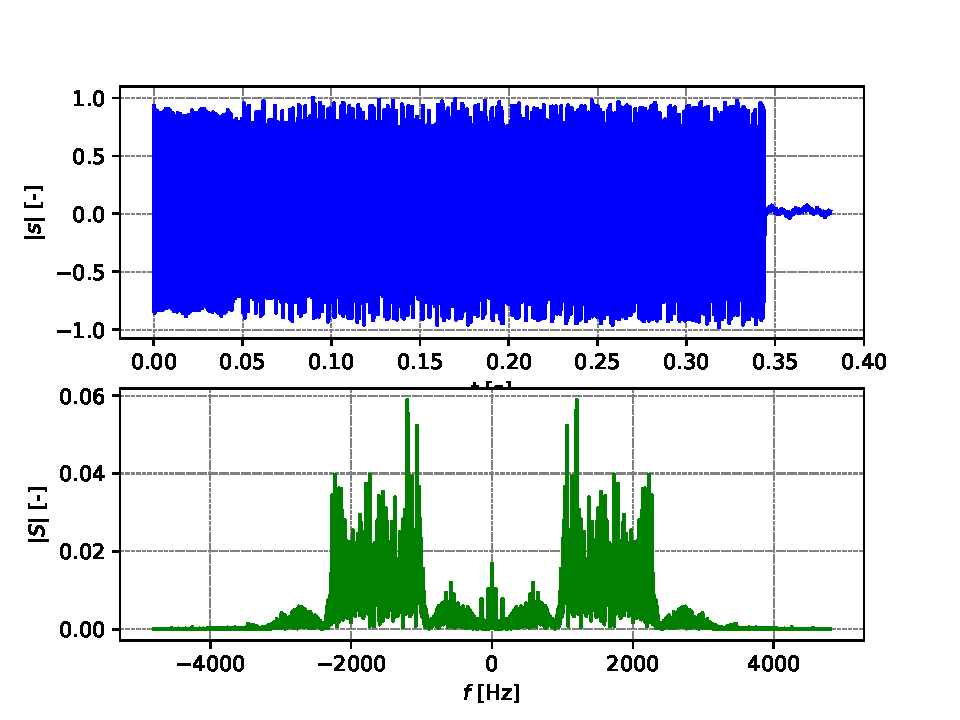
\includegraphics[width=\textwidth]{img/wav.pdf}
    \caption{Časový průběh a frekvenční modulové spektrum vstupního souboru \texttt{1.wav}}
\end{figure}

Jak je ve spektru vidět, nejvíce jsou zastoupeny kmitočty okolo $1,2~kHz$ a $2,2~kHz$, zároveň je v signálu i značné množství šumu.